\subsubsection{Other industries}

This sector is called \textit{other industries}, which one might misunderstand at the first glance. We wanted to be consistent with the sector distribution we found, where this sector is labeled other industry. Actually, it simply refers to all industry except \textit{power industry}.

\paragraph{Strategy}
After conducting some research on how to find suitable indicators for this sector, we found out that global steel production fits our needs. Monthly data is readily available and data researchers are able to predict a country's economic growth with it~\cite{Ravazzolo2020}.
Furthermore, \textit{Le Quéré et al.} model monthly \co data of the industry sector using US steel production data as well~\cite{LeQuere2020}.

\paragraph{Data}
We found recent data of worldwide steel production from January 2019 on, depicted in \autoref{fig:steelallcountries}.
For a longer period of time, we found US steel production data. As shown in \autoref{fig:steelUS}, it ranges from mid 2015 until mid 2020.
\begin{figure}[hbt]
	\centering
	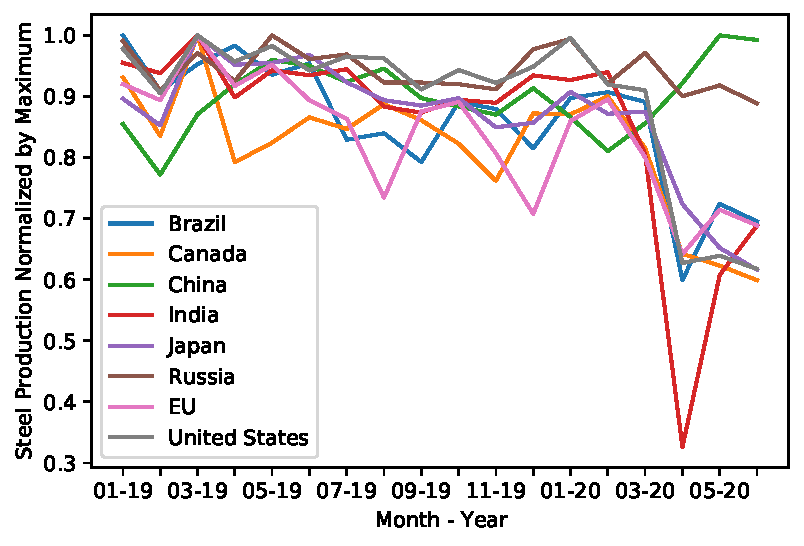
\includegraphics[width=0.69\linewidth]{../predictions/steelAllCountries.pdf}
	\caption{Steel output of all eight countries considered, normalized by the respective maximum for a better comparison.}
	\label{fig:steelallcountries}
\end{figure}

\begin{figure}[hbt]
	\centering
	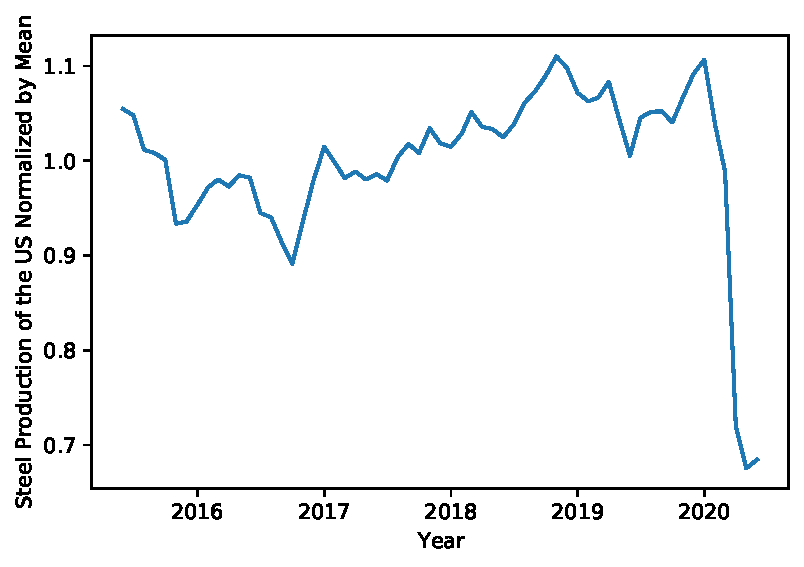
\includegraphics[width=0.69\linewidth]{../predictions/steelUS.pdf}
	\caption{Steel output of the US, normalized by the mean in the years 2015 to 2020.}
	\label{fig:steelUS}
\end{figure}

\newpage

\paragraph{Method}
In contrast to \textit{Le Quéré et al.}, we wanted to use each country's own steel production and not only US data. However, only recent data from 2019 until now is available for free for every country considered in this work. Obviously, one can not find seasonality trends from that. Thus, we use the recent data we have to find a preliminary indicator without seasonality adjustments for each country first, as depicted in \autoref{fig:otherindustry_notadjusted}. For this, we took the early 2020 data of this month and divided it by the early 2020 data and thus obtain a percentage of the steel production output in early 2020 compared to early 2019. 

We then use US steel production data to find a seasonality trend. Furthermore, we assume here that we can transfer this seasonality adjustment to all other countries as well. Our strategy to find a seasonality trend begins with finding mean values of steel production in a given year. We assume that these mean values centered on a given time-point, are the steel production values with seasonality removed. The ratio of the new value without the seasonality effect to the old value is the seasonality trend. Since we can calculate the trend for four different years by using the US data, and we do not want to overfit for a single year, we take the average of seasonality trends of 4 years. Seasonally adjusted steel output of the US can be seen in \autoref{fig:steelUS_adjusted}

\paragraph{Results and conclusion}
As seen in \autoref{tab:otherindustry_seasonality}, our calculated seasonality effect is relatively weak, thus adjusting the data does not have a significant impact. This may also be caused by the limited data.
We can see that for most countries a drop in \co emissions for the \textit{other industries} sector can be expected. For China however, we see more or less stable emissions. This surprised us at first. But the stable steel output can be explained with the fact that COVID-19 only hit a very confined region of China in the beginning and was contained more or less successfully later.

\begin{figure}[hbt]
	\centering
	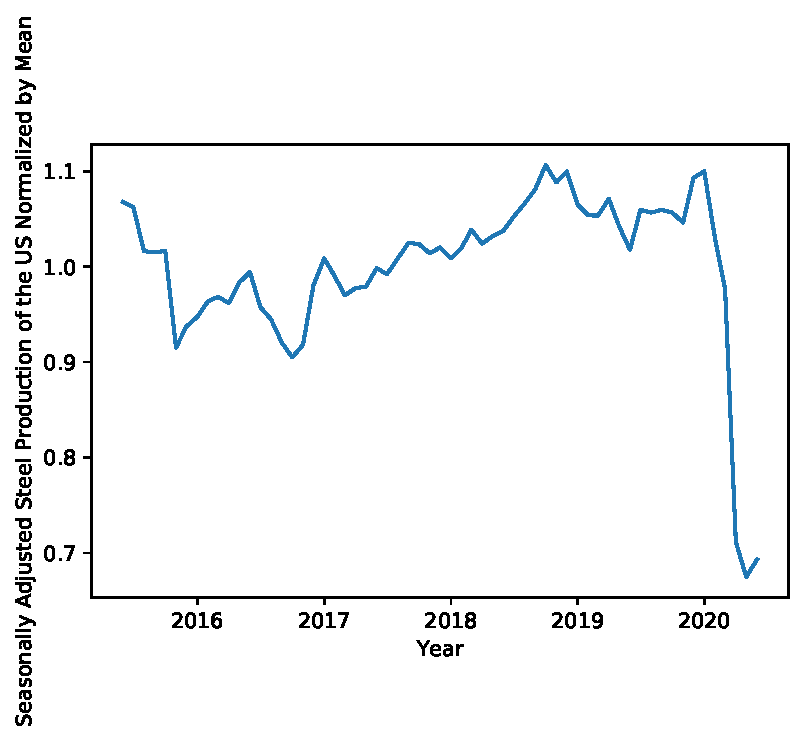
\includegraphics[width=0.69\linewidth]{../predictions/steelUS_seasonadjusted.pdf}
	\caption{Seasonally adjusted steel output of the US, normalized by the mean in the years 2015 to 2020.}
	\label{fig:steelUS_adjusted}
\end{figure}


\begin{table}[h!]
	\centering
	\begin{tabular}{cccccccccccc}
		\hline
		January & February & March & April & May & June & July & August & September & October & November & December\\
		\hline
		\hline
		0.995 & 0.993 & 0.989 & 0.99 & 1.0 & 1.014 & 1.015 & 1.006 & 1.008 & 1.017 & 0.982 & 1.003\\
		\hline &&&&&&&&&&& \\
	\end{tabular}
	\caption{Seasonality trend of steel production in the US.}%todo: source
	\label{tab:otherindustry_seasonality}
\end{table}

\begin{figure}[h]
	\centering
	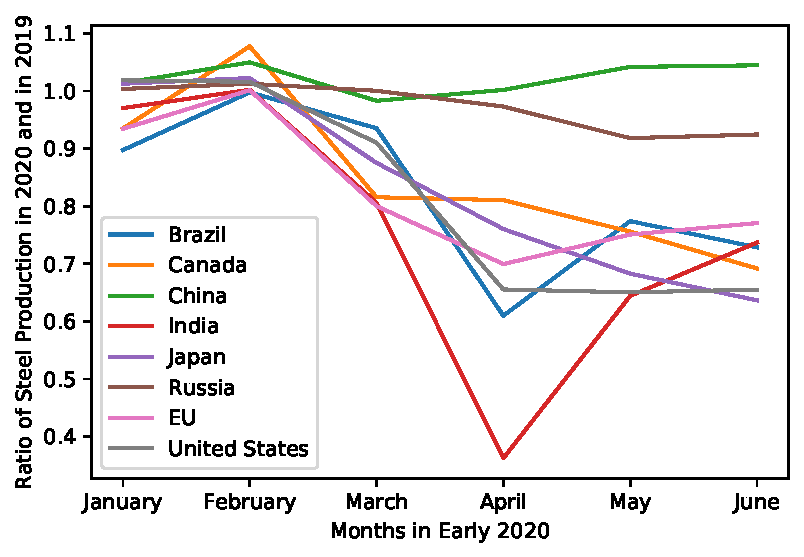
\includegraphics[width=0.7\linewidth]{../predictions/otherindustries_notadjusted.pdf}
	\caption{The indicator of each country without seasonality adjustments.}
	\label{fig:otherindustry_notadjusted}
\end{figure}
